\section{Save\slash Load}
A key feature of this package is the ability to save annotations made to an image and load them automatically when viewing it later. To do this the program saves the locations of every vertex, along with the name of each annotation, within an XML file.  This XML file is stored within the same directory in which the original image resides and the data loaded back when the user reopens that image file.

The XML format was chosen for saving the annotations for two reasons. First, we needed a standard method of storing the meta-data of the image and the widely adopted format for this is XML: probably the main reason for this is that XML can easily inter-operate with multiple applications.  The other reason XML was chosen was that we wanted to make the stored information human-readable, so that when the file is opened in a text editor the user can read and edit the annotations themselves if they so desire.

The image annotation program loads the meta-data of every image automatically, if the appropriate XML file exists in the same directory under the name of that image. This scheme of storing information was chosen to prevent making databases of labels. This has some advantages and disadvantage. One advantage is that there is no need to fetch and alter the labels of a specific image; depending upon the schema of a database, this can be computationally expensive if large numbers of images are considered. Also this method keeps the security of the meta-data at the same level as the images themselves, so when a user does not have access to an image they will not be able to read the annotations either.  By extension, if the user has read-only access they will only be able to read the annotations too. A drawback of this method of storing information is that it would not be easy to implement other features such as search; however, since the use case of this package does not cover it this method was deemed most appropriate.

Many software applications also check for user changes to current file each time a new image is being opened or application is going to close. In our implementation of this feature each time user adds or removes a label or when an annotation is moved, program stores these changes and when a new image is to be opened or when application is closing, asks user whether it should save them or not, Figure \ref{fig:saveview}.

\begin{figure}[h]
\centering
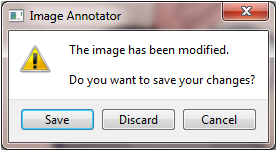
\includegraphics[width=6cm]{save_changes.png}
\caption{A screen-shot of Model window that informs user there are unsaved changes.}
\label{fig:saveview}
\end{figure}

An example file produced by the application can be found in listing \ref{lst:svd} below.    

\begin{center}
\lstset{language=XML, basicstyle=\footnotesize\ttfamily, caption=XML file used to store image labels,frame=single,captionpos=b,label=lst:svd}
\lstinputlisting{svd.txt}
\end{center}
